\section{The Problem}
\begin{frame}
\begin{itemize}
  \item % TODO What is the problem and why do we care
\end{itemize}
\end{frame}

\subsection{Background}
\begin{frame}{Pig Latin Compilation}
\begin{itemize}
	\item Parser verifies the programs, performs type checking, schema inference and other tasks.
	\item It outputs a canonical logical plan.
	\item The logical plan is optimized and compiled to a series of Map-Reduce Jobs.
	\item The DAG of optimized Map-Reduce jobs are sorted topologically and jobs are submitted to Hadoop for execution. 
\end{itemize}
\end{frame}

\subsection{MapReduce}
\begin{frame}{Execution Model}
\begin{itemize}
	\item Map: Produces a stream of data items annotated with keys.
	\item Local Sort: Orders the data at each machine by key.
	\item Combiner: Performs partial aggregation on the locally ordered data.
	\item Shuffle: Redistributes the data to achieve global ordering.
	\item Merge/Combine: All data received at a particular machine is combined to into a single stream in merge stage.
	\item Reduce: Finally the reduce stage processes the data associated with each key and performs aggregation of the output results.
\end{itemize}
\end{frame}

\begin{frame}{MapReduce Execution Model}
\centerline{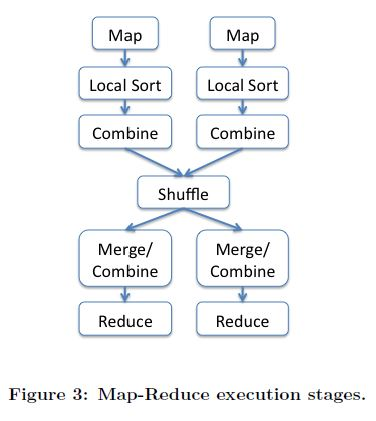
\includegraphics[scale=0.5]{Images/MapReduce_Execution.JPG}}
\let\thefootnote\relax\footnotetext{\tiny The Pig Experience - Gates et al.} 
\end{frame}

\subsection{Pig Latin Compilation}
\begin{frame}{Logical Plan Structure}
\begin{itemize}
	\item A Pig Latin program is a sequence of steps, each of which carries out a single transformation.
	\item Each Pig Latin program is translated to a logical plan
	\item Pig then translates the logical plan to a physical plan and embeds each physical operator inside a Map-Reduce stage to arrive at the Map-Reduce plan.
\end{itemize}
\end{frame}

\begin{frame}{PigLatin - Logical Plan}
\centerline{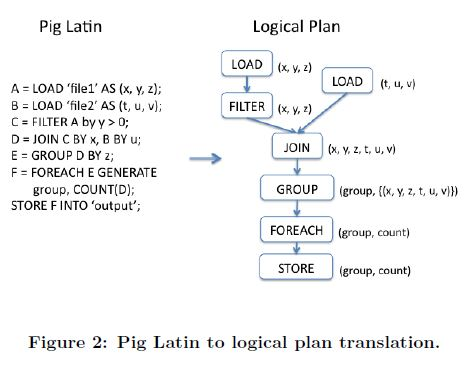
\includegraphics[scale=0.55]{Images/PigLatin.JPG}}
\let\thefootnote\relax\footnotetext{\tiny The Pig Experience - Gates et al.}
\end{frame}

\subsection{Generating MapReduce Jobs}
\begin{frame}{Logical-MapReduce}
\begin{itemize}
	\item Pig translates the logical plan to a physical plan
	\item Logical (CO)GROUP operator translates to - local rearrange, global rearrange and package.
	\item The JOIN is handled either with a COGROUP followed by a FOREACH or fragment replicate join.
	\item After the physical plan is generated Pig assigns physical operators to Hadoop Stages
\end{itemize}
\end{frame}

\begin{frame}
\centerline{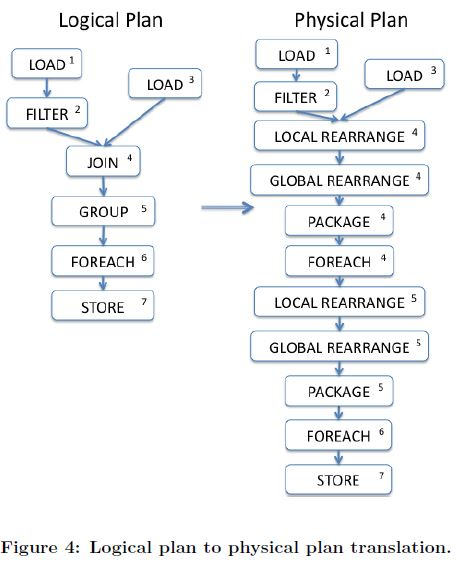
\includegraphics[scale=0.45]{Images/Logical_Physical.JPG} }
\let\thefootnote\relax\footnotetext{\tiny The Pig Experience - Gates et al.}
\end{frame}

\begin{frame}
\centerline{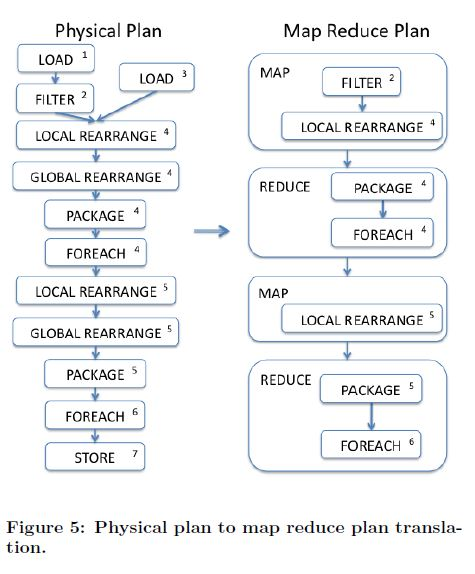
\includegraphics[scale=0.45]{Images/Physical_MapReduce.JPG}}
\let\thefootnote\relax\footnotetext{\tiny The Pig Experience - Gates et al.}
\end{frame}

\begin{frame}
\begin{itemize}
	\item Pig compiles programs written in Pig Latin
	\item Ultimately translates to Map-Reduce tasks
	\item Pig also operates on local mode running on a single machine without map-reduce
	\item There lies an equivalence between PigLatin and MapReduce operational semantics
	\item The equivalence needs to be formalized and correctness needs to be proved  
\end{itemize}
\end{frame}